%%%%%%%%%%%%%%%%%%%%%%%%%%%%%%%%%%%%%%%%%%%%%%%%%%%%%%%%
%   |------------------------------------------|       %
%   | Web App embebida en dispositivos móviles |       %
%   |  para la gestión de registros sobre la   |       %
%   |   contaminación de afluentes y ríos.     |       %
%   |                                          |       %
%   |          Proyecto de graduación          |       %
%   |__________________________________________|       %
%                                                      %
%   Autores                                            %
%   -------                                            %
%                                                      %
% * Bruno, Ricardo Hugo (CX 1409686)                   %
%     rburnount@gmail.com                              %
% * Gomez Veliz, Kevin Shionen (CX 1411828)            %
%     ing.gomezvelizkevin@gmail.com                    %
%                                                      %
%   Tutor                                              %
%   -------                                            %
%                                                      %
% * Ing. Cohen, Daniel Eduardo                         %
%        dcohen.tuc@gmail.com                          %
%                                                      %
%   Cotutor                                            %
%   -------                                            %
%                                                      %
% * Ing. Nieto, Luis Eduardo                           %
%        lnieto@herrera.unt.edu.ar                     %
%                                                      %
%                                                      %
%%%%%%%%%%%%%%%%%%%%%%%%%%%%%%%%%%%%%%%%%%%%%%%%%%%%%%%%

\chapter{Disciplina de Análisis}
\label{chap:analisis}

\section{Vista de Casos de Uso}

La vista de casos de uso captura el comportamiento de un sistema, subsistema, clase o componente, como lo ve un usuario externo. Particiona la funcionalidad del sistema en transacciones significativas para los actores (usuarios idealizados) de un sistema. Las piezas de funcionalidad interactiva son llamadas ``casos de uso''. Un caso de uso describe una interacción entre actores como una secuencia de mensajes entre el sistema y uno o más actores. El término \emph{actor} incluye a personas, como también otros sistemas de computadora o procesos.

\section{Diagrama de Contexto}

\begin{figure}[H]
  \centering
   
    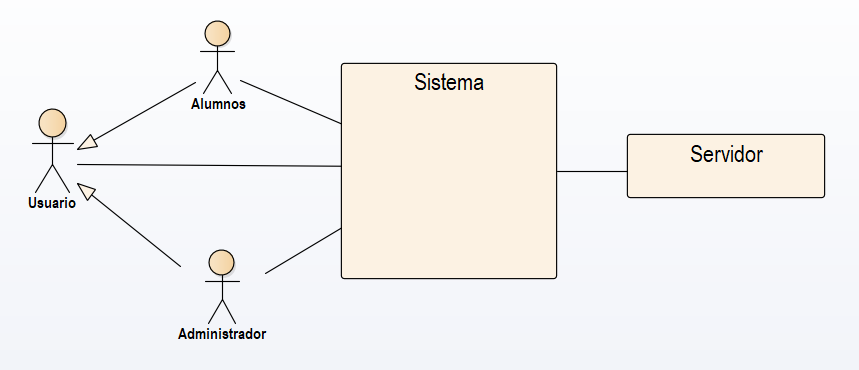
\includegraphics[width=1\textwidth]{imagenes/analisis/diagrama-contexto.png}
        %%Me parece que queda mejor sin el hfill
        %\hfill
    %\caption{epígrafe}
	\label{fig:casos-de-uso}
\end{figure}

\section{Diagramas de Casos de Uso}

\subsection{Diagrama de Casos de Uso general}

\begin{figure}[H]
  \centering
    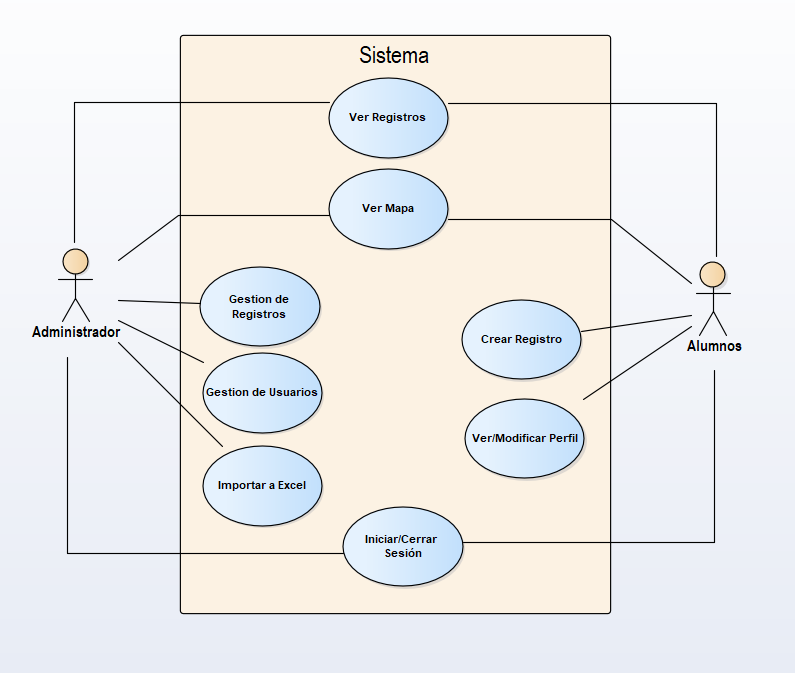
\includegraphics[width=0.7\textwidth]{imagenes/analisis/casos-uso-general.png}
        %%Me parece que queda mejor sin el hfill
        %\hfill
	%\caption{epígrafe}
	\label{fig:casos-de-uso}
\end{figure}

\subsection{Diagrama de Casos de Uso de gestión de usuarios}

\begin{figure}[H]
  \centering
    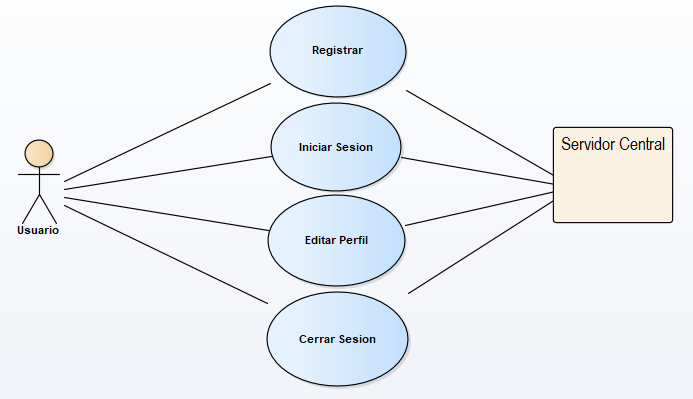
\includegraphics[width=0.7\textwidth]{imagenes/analisis/casos-uso-usuario.png}
        %%Me parece que queda mejor sin el hfill
        %\hfill
    %\caption{epígrafe}
	\label{fig:casos-de-uso-usuario}
\end{figure}

\subsection{Diagrama de Casos de Uso de gestión de tienda}

\begin{figure}[H]
  \centering
    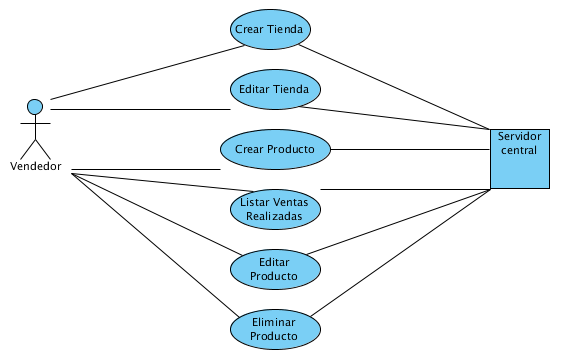
\includegraphics[width=0.7\textwidth]{imagenes/analisis/casos-uso-tienda.png}
        %%Me parece que queda mejor sin el hfill
        %\hfill
    %\caption{epígrafe}
    \label{fig:casos-de-uso-tienda}
\end{figure}


\section{Diagramas de Actividad}

\subsection{Autenticar}
\begin{figure}[H]
  \centering
    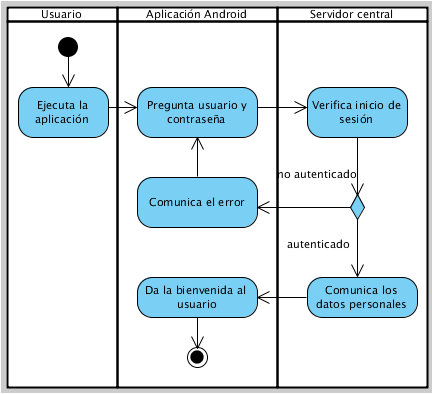
\includegraphics{imagenes/analisis/diagrama-actividad-autenticar.png}
        %%Me parece que queda mejor sin el hfill
        %\hfill
    \label{fig:diagrama-actividad-autenticar}
\end{figure}

\subsection{Registrar}

\begin{figure}[H]
  \centering
    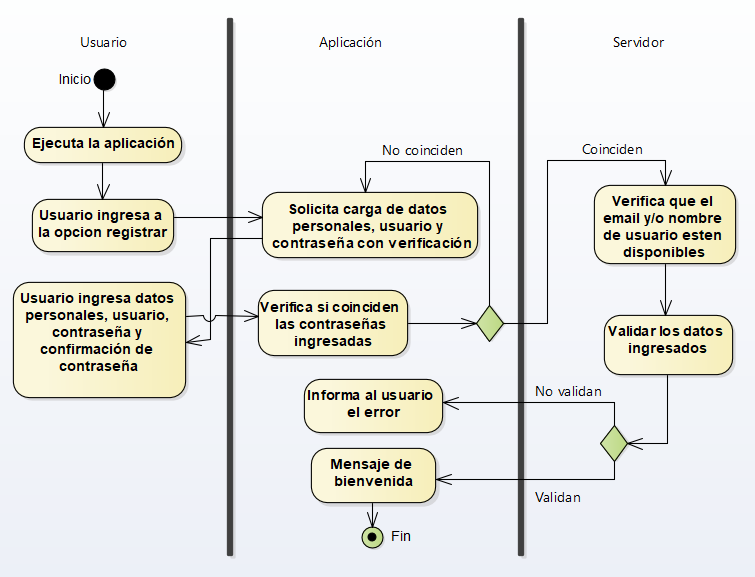
\includegraphics[width=1\textwidth]{imagenes/analisis/diagrama-actividad-registrar.png}
        %%Me parece que queda mejor sin el hfill
        %\hfill
	\label{fig:diagrama-actividad-registrar}
\end{figure}

\subsection{Crear Tienda}

\begin{figure}[H]
  \centering
    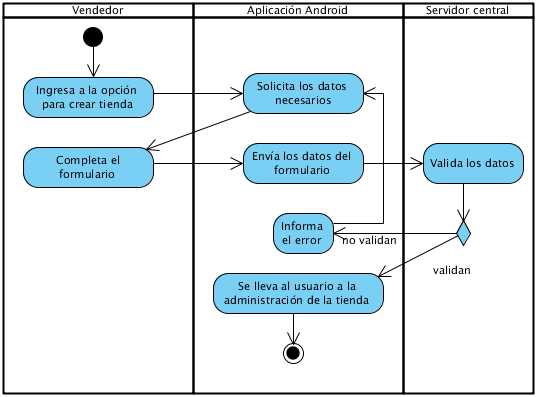
\includegraphics{imagenes/analisis/diagrama-actividad-crear-tienda.png}
        %%Me parece que queda mejor sin el hfill
        %\hfill
    \label{fig:diagrama-actividad-crear-tienda}
\end{figure}

\subsection{Comprar Producto}

\begin{figure}[H]
  \centering
    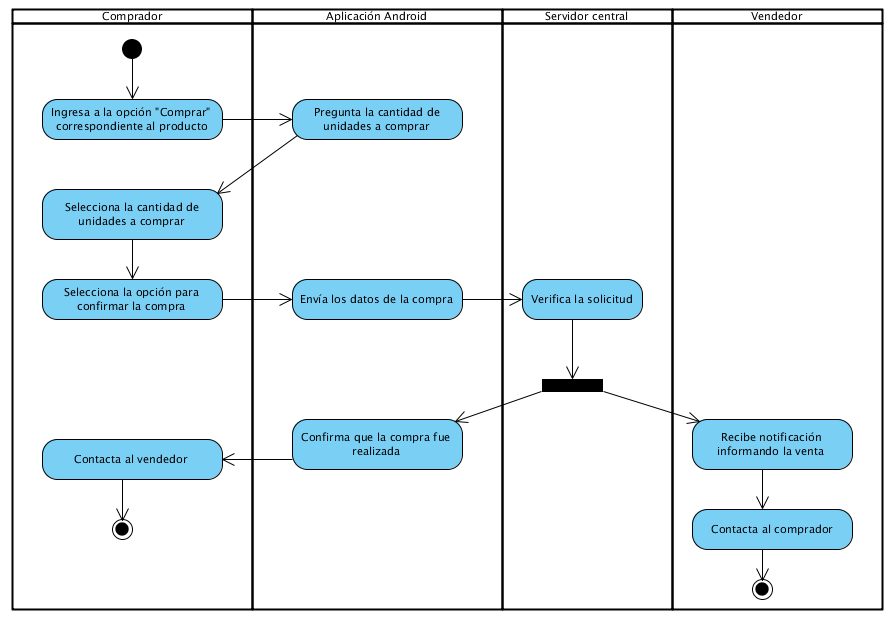
\includegraphics[width=1\textwidth]{imagenes/analisis/actividad-comprar-producto.png}
        %%Me parece que queda mejor sin el hfill
        %\hfill
    \label{fig:diagrama-actividad-comprar-producto}
\end{figure}


\section{Diagrama de Clases del Dominio}

\begin{figure}[H]
  \centering
    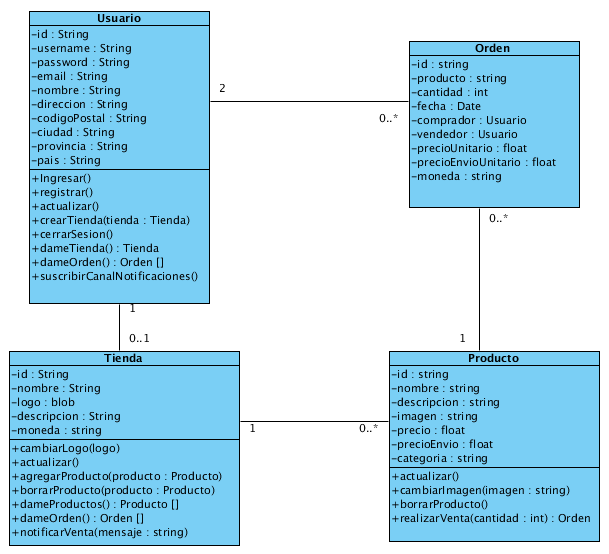
\includegraphics[width=0.9\textwidth]{imagenes/analisis/clases-dominio.png}
        %%Me parece que queda mejor sin el hfill
        %\hfill
    %\caption{epígrafe}
    \label{fig:clases-dominio}
\end{figure}